\documentclass[11pt,aspectratio=169]{beamer}

\usetheme{metropolis}
\usepackage[utf8]{inputenc}
\usepackage[T1]{fontenc}
\usepackage{booktabs}
\usepackage{tikz}
\usetikzlibrary{shapes.geometric, arrows.meta, positioning, calc}
\usepackage{array}

\definecolor{mathblue}{RGB}{41,98,158}
\definecolor{aicoral}{RGB}{214,93,74}
\definecolor{aipurple}{RGB}{130,90,160}
\definecolor{softgray}{RGB}{110,110,110}
\definecolor{darkbg}{RGB}{30,33,36}

\setbeamercolor{palette primary}{bg=mathblue, fg=white}
\setbeamercolor{frametitle}{bg=mathblue, fg=white}
\setbeamercolor{progress bar}{fg=aicoral, bg=softgray!25}
\setbeamercolor{alerted text}{fg=aicoral}
\setbeamertemplate{frame footer}{}
\metroset{sectionpage=progressbar, numbering=fraction}

\title{Construction d'un arbre hiérarchique hybride}
\subtitle{Génération de code frontend à partir de maquettes UX \\ \small Point d'avancement méthodologique}
\author{}
\date{}

\begin{document}

\maketitle

\begin{frame}{Sommaire}
  \tableofcontents
\end{frame}

\section{Contexte et objectif}

\begin{frame}{Le pipeline général}
  \begin{center}
  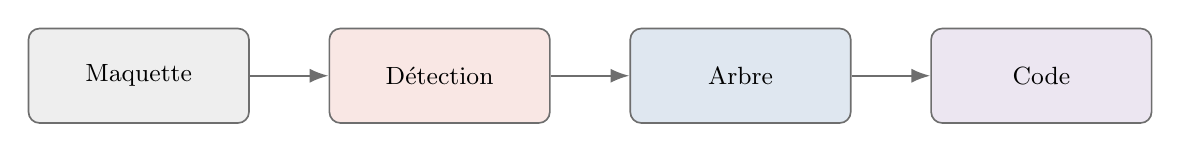
\begin{tikzpicture}[
    box/.style={rectangle, rounded corners=4pt, draw=softgray, line width=0.6pt,
                minimum width=2.8cm, minimum height=1.2cm, align=center, font=\small},
    arr/.style={-{Latex[length=2.4mm]}, line width=0.8pt, draw=softgray}
  ]
  \node[box, fill=softgray!12] (m) {Maquette};
  \node[box, fill=aicoral!15, right=1cm of m] (d) {Détection};
  \node[box, fill=mathblue!15, right=1cm of d] (a) {Arbre};
  \node[box, fill=aipurple!15, right=1cm of a] (c) {Code};
  \draw[arr] (m) -- (d);
  \draw[arr] (d) -- (a);
  \draw[arr] (a) -- (c);
  \end{tikzpicture}
  \end{center}
  \vspace{6mm}
  \begin{center}
  \begin{minipage}{0.85\textwidth}
  \centering
  Toute méthode passe par un modèle structuré intermédiaire : \alert{l'arbre hiérarchique}. \\[4pt]
  \small La qualité du code final dépend presque entièrement de la qualité de cet arbre.
  \end{minipage}
  \end{center}
\end{frame}

\begin{frame}{Objectif du mémoire}
  \begin{itemize}
    \item Se concentrer sur l'étape la plus fragile du pipeline : \alert{la construction de l'arbre}
    \item Proposer une méthode \textbf{hybride}, combinant précision géométrique et compréhension sémantique
    \item Livrables : un article de recherche \textbf{et} sa soutenance orale
  \end{itemize}
\end{frame}

\section{Le problème de recherche}

\begin{frame}{Deux familles, deux défauts opposés}
  \begin{columns}[T,onlytextwidth]
    \begin{column}{0.48\textwidth}
      \begin{alertblock}{Modèles multimodaux (MLLM)}
        Comprennent bien le \textbf{sens} des éléments \\[2pt]
        \alert{Hallucinent leur position} exacte
      \end{alertblock}
    \end{column}
    \begin{column}{0.48\textwidth}
      \begin{block}{Méthodes mathématiques}
        Précises sur la \textbf{position} \\[2pt]
        \alert{Aveugles au sens} des éléments
      \end{block}
    \end{column}
  \end{columns}
  \vspace{8mm}
  \begin{center}
  \small Aucun travail existant ne sépare complètement et strictement ces deux rôles.
  \end{center}
\end{frame}

\section{État de l'art étudié}

\begin{frame}{Trois travaux de référence}
  \small
  \renewcommand{\arraystretch}{1.6}
  \begin{tabular}{@{}p{2.1cm}p{3.6cm}p{5.6cm}@{}}
    \toprule
    \textbf{Travail} & \textbf{Approche} & \textbf{Limite identifiée} \\
    \midrule
    DeclarUI & Vision par ordinateur + MLLM & Échoue sur les regroupements complexes (sections, listes) ; centré sur la navigation entre pages \\
    ReverseORC & Découpage géométrique récursif (XY-Cut), depuis API d'accessibilité & Aucune étape sémantique ; ne part pas d'une image \\
    DesignCoder & Arbre construit par l'IA en premier, géométrie calculée ensuite & Ordre inverse du nôtre ; dépend de métadonnées déjà connues \\
    \bottomrule
  \end{tabular}
\end{frame}

\begin{frame}{Le vide identifié}
  \begin{center}
  \Large Aucune méthode ne garantit à la fois : \\[6mm]
  \begin{columns}[T,onlytextwidth]
    \begin{column}{0.5\textwidth}
      \centering
      \large \textcolor{mathblue}{\textbf{100\% de précision}}\\ \small sur les positions
    \end{column}
    \begin{column}{0.5\textwidth}
      \centering
      \large \textcolor{aicoral}{\textbf{une vraie compréhension}}\\ \small des sections et listes complexes
    \end{column}
  \end{columns}
  \end{center}
\end{frame}

\section{Notre proposition}

\begin{frame}{Une séparation stricte en deux temps}
  \begin{center}
  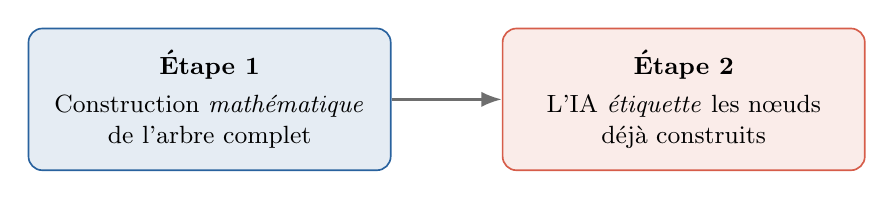
\begin{tikzpicture}[
    node distance=10mm and 14mm,
    box/.style={rectangle, rounded corners=5pt, draw=softgray, line width=0.6pt,
                minimum width=4.6cm, minimum height=1.8cm, align=center, font=\small},
    mathbox/.style={box, fill=mathblue!12, draw=mathblue},
    aibox/.style={box, fill=aicoral!12, draw=aicoral},
    arr/.style={-{Latex[length=2.6mm]}, line width=0.9pt, draw=softgray}
  ]
  \node[mathbox] (math) {\textbf{Étape 1}\\[3pt] Construction \emph{mathématique}\\ de l'arbre complet};
  \node[aibox, right=of math] (ai) {\textbf{Étape 2}\\[3pt] L'IA \emph{étiquette} les nœuds\\ déjà construits};
  \draw[arr] (math) -- (ai);
  \end{tikzpicture}
  \end{center}
  \vspace{6mm}
  \begin{center}
  \alert{L'IA ne modifie jamais une position} --- elle attache seulement un nom. \\[4pt]
  \small C'est l'inverse exact de l'ordre choisi par DesignCoder.
  \end{center}
\end{frame}

\begin{frame}{Pourquoi cet ordre}
  \begin{itemize}
    \item Le calcul garantit une structure \textbf{fiable et déterministe}
    \item L'IA n'a plus qu'un seul rôle simple : \textbf{nommer}, jamais positionner
    \item Les erreurs de raisonnement du MLLM ne peuvent plus contaminer la géométrie
    \item Approche \textbf{nouvelle}, pas une amélioration incrémentale d'un travail existant
  \end{itemize}
\end{frame}

\begin{frame}{Deux niveaux d'ambition pour l'étiquetage}
  \begin{columns}[T,onlytextwidth]
    \begin{column}{0.48\textwidth}
      \begin{block}{Option A --- priorité}
        Étiquetage sémantique simple de chaque nœud déjà construit
      \end{block}
    \end{column}
    \begin{column}{0.48\textwidth}
      \begin{alertblock}{Option B --- bonus}
        Détecter les sous-arbres similaires \\ $\rightarrow$ composants réutilisables
      \end{alertblock}
    \end{column}
  \end{columns}
  \vspace{6mm}
  \small \centering L'Option A est développée et validée en premier pour garantir un résultat défendable dans les délais.
\end{frame}

\section{Détection : une entrée image seule}

\begin{frame}{Contrainte choisie}
  \begin{itemize}
    \item Le pipeline ne reçoit \textbf{que la capture d'écran} haute fidélité --- aucune métadonnée de conception (Figma ou autre)
    \item Contrairement à ReverseORC (API d'accessibilité) et DesignCoder (métadonnées id/bbox/type/style), notre entrée reste une image pure
    \item Un éventuel code source réel ne sert que de \textbf{vérité terrain} pour l'évaluation --- jamais donné au pipeline
  \end{itemize}
\end{frame}

\begin{frame}{Détecteur spécialisé plutôt qu'un MLLM}
  \begin{columns}[T,onlytextwidth]
    \begin{column}{0.48\textwidth}
      \begin{block}{Détecteur spécialisé}
        Analyse des pixels, sans raisonnement \\[2pt]
        Position \textbf{fiable et déterministe}
      \end{block}
    \end{column}
    \begin{column}{0.48\textwidth}
      \begin{alertblock}{MLLM pour la détection}
        \alert{Hallucine les positions}, comme identifié dès le départ
      \end{alertblock}
    \end{column}
  \end{columns}
  \vspace{8mm}
  \begin{center}
  \small Utiliser un MLLM ici casserait notre principe fondateur : la géométrie doit rester garantie par le calcul.
  \end{center}
\end{frame}

\begin{frame}{Preuve : le MLLM peut déterminer un type sémantique}
  \begin{itemize}
    \item \textbf{DesignCoder} \cite{designcoder} : à partir d'un élément déjà localisé (bbox connue), un prompt dédié fait produire au MLLM une description sémantique précise --- ex.\ un champ de recherche annoté comme suggérant \textit{``search scope''}
    \item \textbf{ScreenCoder} \cite{screencoder} : son agent interroge le MLLM (\textit{``Where is the sidebar?''}) qui renvoie une région \textbf{et} son étiquette
  \end{itemize}
  \vspace{4mm}
  \small \textit{Nuance : ScreenCoder utilise le MLLM aussi pour la position --- l'inverse de notre choix. Ses propres mécanismes de correction (NMS, heuristiques de secours) montrent que ce choix reste risqué sur la position.}
\end{frame}

\begin{frame}{Détecteurs utilisés dans la littérature}
  \small
  \renewcommand{\arraystretch}{1.5}
  \begin{tabular}{@{}p{2.6cm}p{4.4cm}p{4.6cm}@{}}
    \toprule
    \textbf{Travail} & \textbf{Détecteur} & \textbf{Ce qu'il fournit} \\
    \midrule
    DeclarUI \cite{declarui} & Détection non supervisée + SAM & Régions, sans type direct \\
    Vu et al. \cite{multimodalgraph} & OCR puis SAM & Texte typé, régions visuelles non typées \\
    Screen Parsing \cite{screenparsing} & Faster R-CNN entraîné sur UI (AMP/RICO) & \alert{Position + type en une passe} \\
    ScreenCoder \cite{screencoder} & MLLM (grounding) & Position + type, mais non géométrique \\
    \bottomrule
  \end{tabular}
\end{frame}

\begin{frame}{Quel détecteur pour notre cas ?}
  \begin{block}{Notre besoin précis}
    Un détecteur qui fournit \textbf{position + type grossier en une seule passe}, sans MLLM
  \end{block}
  \vspace{4mm}
  \begin{itemize}
    \item DeclarUI et Vu et al. reposent sur \textbf{SAM} : segmentation fiable, mais \alert{aucun type} n'est produit --- une étape supplémentaire serait nécessaire
    \item \textbf{Screen Parsing} \cite{screenparsing} entraîne directement un détecteur d'objets (Faster R-CNN) à sortir des \textit{``class-labeled bounding boxes''} --- position et type en une seule passe, exactement notre besoin
  \end{itemize}
  \vspace{4mm}
  \begin{center}
  \alert{\textbf{Piste retenue}} : un détecteur entraîné de type Faster R-CNN, sur le modèle de Screen Parsing
  \\[2pt]
  \small \textit{Limite à garder en tête : entraîné sur des interfaces mobiles (AMP/RICO) --- à vérifier sur des maquettes web}
  \end{center}
\end{frame}

\begin{frame}[allowframebreaks]{Bibliographie}
  \small
  \begin{thebibliography}{9}
  \bibitem{declarui} Zhou, T. et al. \textit{Bridging design and development with automated declarative UI code generation.} arXiv:2409.11667, 2024.
  \bibitem{designcoder} Chen, Y. et al. \textit{DesignCoder: Hierarchy-Aware and Self-Correcting UI Code Generation with LLMs.}
  \bibitem{reverseorc} Jiang, Y., Stuerzlinger, W., Lutteroth, C. \textit{ReverseORC: Reverse Engineering of Resizable UI Layouts with OR-Constraints.} CHI 2021.
  \bibitem{screenparsing} Wu, J. et al. \textit{Screen Parsing: Towards Reverse Engineering of UI Models from Screenshots.} UIST 2021.
  \bibitem{multimodalgraph} Vu, T.D., Hoang, C., Hy, T.S. \textit{Multimodal Graph Representation Learning for Website Generation Based on Visual Sketch.} arXiv:2504.18729.
  \bibitem{screencoder} Jiang, Y. et al. \textit{ScreenCoder: Advancing Visual-to-Code Generation via Modular Multimodal Agents.} arXiv:2507.22827.
  \end{thebibliography}
\end{frame}

\begin{frame}{Ce que fournit le détecteur retenu}
  \begin{itemize}
    \item Une \textbf{position exacte} (bbox) pour chaque élément
    \item Un \textbf{type grossier} : Texte / Image / Composant --- \textbf{en une seule passe}, sans étape supplémentaire
    \item Rien de plus --- aucune compréhension du sens
  \end{itemize}
\end{frame}

\begin{frame}{Le rôle du MLLM reste central}
  \begin{center}
  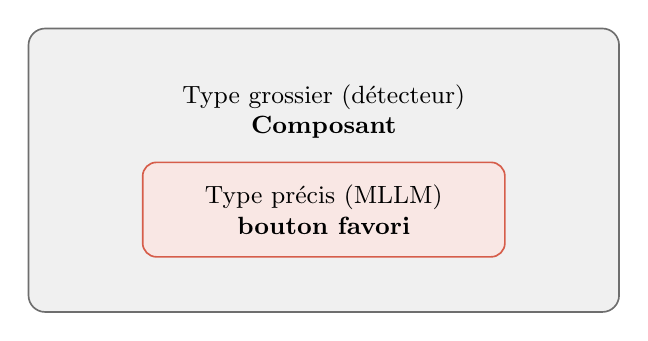
\begin{tikzpicture}[
    outer/.style={rectangle, rounded corners=6pt, draw=softgray, fill=softgray!10, line width=0.6pt, minimum width=7.5cm, minimum height=3.6cm},
    inner/.style={rectangle, rounded corners=5pt, draw=aicoral, fill=aicoral!15, line width=0.6pt, minimum width=4.6cm, minimum height=1.2cm, align=center, font=\small}
  ]
  \node[outer] (out) {};
  \node[align=center, font=\small, anchor=north] at ([yshift=-6mm]out.north) {Type grossier (détecteur)\\ \textbf{Composant}};
  \node[inner, anchor=south] at ([yshift=7mm]out.south) {Type précis (MLLM)\\ \textbf{bouton favori}};
  \end{tikzpicture}
  \end{center}
  \vspace{4mm}
  \begin{center}
  \small Pas de contradiction : le sens précis du MLLM est \emph{contenu} dans le type grossier, jamais en désaccord avec lui.
  \end{center}
\end{frame}

\begin{frame}{Pourquoi pas de vérification croisée}
  \begin{itemize}
    \item Une vérification détecteur $\leftrightarrow$ MLLM sur le type dirait presque toujours ``d'accord'' --- complexité sans bénéfice réel
    \item Sans le MLLM, l'arbre resterait muet, comme Prototype2Code : bien rangé, mais incapable de dire ce que chaque partie représente
    \item Le MLLM reste \textbf{seul responsable} du sens --- c'est notre contribution centrale, pas un rôle secondaire
  \end{itemize}
\end{frame}

\section{Avancement et prochaines étapes}

\begin{frame}{Où nous en sommes}
  \begin{enumerate}
    \item \textcolor{mathblue}{\textbf{Cadrage du sujet}} --- terminé \checkmark
    \item \textcolor{mathblue}{\textbf{Choix de la stratégie de détection}} --- terminé \checkmark
    \item \alert{\textbf{Définition formelle de la structure de l'arbre}} --- en cours
    \item Construction de l'algorithme géométrique
    \item Intégration de l'étiquetage sémantique
    \item Préparation des données de test
    \item Mesure des résultats
    \item Rédaction de l'article
    \item Relecture et finalisation
  \end{enumerate}
\end{frame}

\begin{frame}{Prochaine étape}
  \begin{center}
  \Large Définir précisément ce que doit contenir\\ un \alert{nœud} de notre arbre
  \\[6mm]
  \small en s'appuyant sur les structures déjà étudiées \\ (ReverseORC, DesignCoder)
  \end{center}
\end{frame}

\begin{frame}[standout]
  Merci --- questions et retours bienvenus
\end{frame}

\end{document}
